\subsection{Collie River Basin 2 (model ID: 03)}
The Collie River Basin 2 model (fig.~\ref{fig:03_schematic}) is part of a top-down modelling exercise and is originally applied at the monthly scale \citep{Jothityangkoon2001}. It has 1 store and 4 parameters ($S_{max}$, $S_{fc}$, $a$, $M$). The model aims to represent:

\begin{itemizecompact}
\item Separate bare soil and vegetation evaporation;
\item Saturation excess surface runoff;
\item Subsurface runoff.
\end{itemizecompact}

\subsubsection{File names}
\begin{tabular}{@{}ll}
Model: &m\_03\_collie2\_4p\_1s \\
Parameter ranges: &m\_03\_collie2\_4p\_1s\_parameter\_ ranges \\
\end{tabular}

% Equations
\subsubsection{Model equations}

% Model layout figure
{ 																	% This ensures it doesn't warp text further down
\begin{wrapfigure}{l}{5cm}
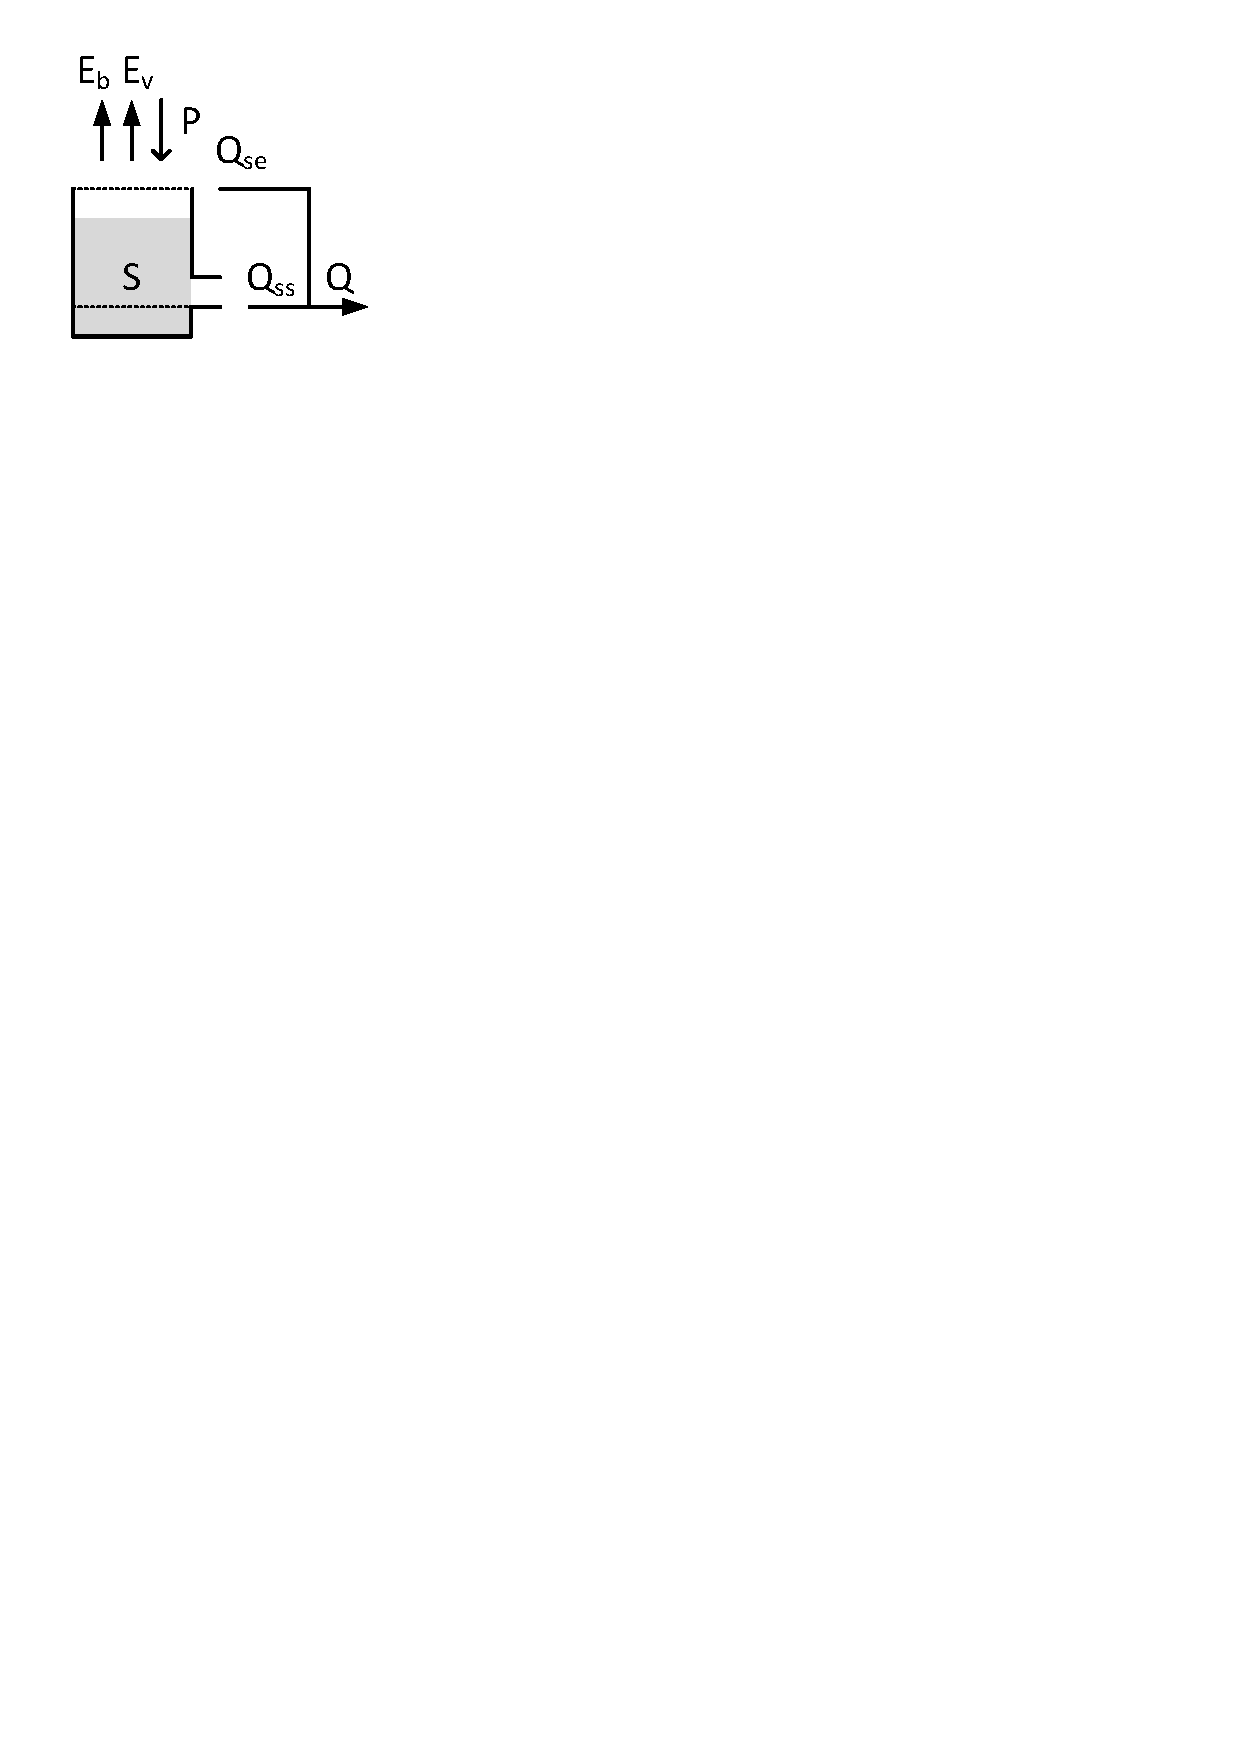
\includegraphics[trim=1cm 24cm 9cm 1cm,keepaspectratio]{./files/03_schematic.pdf}
\caption{Structure of the Collie River Basin 2 model} \label{fig:03_schematic}
\end{wrapfigure}

\begin{align}
	\frac{dS}{dt} &= P -E_b - E_v -Q_{se}-Q_{ss} \\
	Eb &= \frac{S}{S_{max}}(1-M)*Ep\\
	Ev &= 
		\begin{cases}
			M*E_p, & if~S>S_{fc}\\
			\frac{S}{S_{fc}}*M*E_p, &otherwise\\
		\end{cases}\\
	Q_{se} &= 
		\begin{cases}
			P, & if~S>S_{max}\\
			0, & otherwise \\
		\end{cases}\\
	Q_{ss} &= 
		\begin{cases}
			a*(S-S{fc}), & if~S>S_{fc}\\
			0, & otherwise 
		\end{cases}
\end{align}
}
\vspace{0.5cm}

Where $S$ [mm] is the current storage in the soil moisture and $P$ $[mm/d]$ the precipitation input. 
Actual evaporation is split between bare soil evaporation $E_b$ $[mm/d]$ and transpiration through vegetation $E_v$ $[mm/d]$, controlled through the forest fraction $M$ [-]. 
The evaporation estimates are based on the current storage $S$, the potential evapotranspiration $E_p$ $[mm/d]$, maximum soil moisture storage $S_{max}$ [mm] and field capacity $S_{fc}$ [mm] respectively. 
$Q_{se}$ $[mm/d]$ is saturation excess overland flow.  $Q_{ss}$ $[mm/d]$ is subsurface flow regulated by runoff coefficient $a$ $[d^{-1}]$.
Total flow:

\begin{align}
	Q &= Q_{se}+Q_{ss}
\end{align}

\newpage
\subsubsection{Parameter overview}
% Table generated by Excel2LaTeX from sheet 'Sheet1'
\begin{table}[htbp]
  \centering
    \begin{tabular}{lll}
    \toprule
    Parameter & Unit  & Description \\
    \midrule
    $S_{max}$ & $mm$  & Maximum soil moisture storage \\
    $S_{fc}$ & $mm$  & Field capacity \\
    $a$   & $d^{-1}$ & Runoff coefficient \\
    $M$   & $-$   & Forest fraction \\
    \bottomrule
    \end{tabular}%
  \label{tab:addlabel}%
\end{table}%
